\documentclass[12pt,a4paper,oneside]{report}

% ------------------------------------------------------------
% Robo-Matter BTP Report
% Compile with: pdflatex BTP_RoboMatter_Report.tex
% Run twice for the table of contents and cross-references.
% ------------------------------------------------------------

\usepackage[a4paper,margin=1in]{geometry}
\usepackage[T1]{fontenc}
\usepackage[utf8]{inputenc}
\usepackage{lmodern}
\usepackage{microtype}
\usepackage{setspace}
\usepackage{graphicx}
\usepackage{xcolor}
\usepackage{amsmath,amssymb,bm}
\usepackage{booktabs}
\usepackage{tabularx}
\usepackage{longtable}
\usepackage{array}
\usepackage{enumitem}
\usepackage{caption}
\usepackage{float}
\usepackage{fancyhdr}
\usepackage{titlesec}
\usepackage{tikz}
\usepackage[most]{tcolorbox}
\usepackage{listings}
\usepackage[hidelinks]{hyperref}

\graphicspath{{states/}}

\definecolor{ReportBlue}{HTML}{1F4E79}
\definecolor{SoftBlue}{HTML}{EAF2F8}
\definecolor{SoftGreen}{HTML}{EAF7EF}
\definecolor{SoftAmber}{HTML}{FFF4DC}
\definecolor{SoftGray}{HTML}{F5F7FA}
\definecolor{Ink}{HTML}{1F2933}
\definecolor{Muted}{HTML}{5B6770}
\definecolor{AccentGreen}{HTML}{2D7D46}
\definecolor{AccentAmber}{HTML}{A66A00}
\definecolor{AccentPurple}{HTML}{5B4B8A}

\hypersetup{
  colorlinks=true,
  linkcolor=ReportBlue,
  citecolor=ReportBlue,
  urlcolor=ReportBlue,
  hypertexnames=false
}

\setstretch{1.18}
\setlength{\parindent}{0pt}
\setlength{\parskip}{6pt}
\setlength{\headheight}{14pt}
\captionsetup{font=normalsize,labelfont=bf}

\pagestyle{fancy}
\fancyhf{}
\lhead{\small\textcolor{Muted}{Simulation and Analysis of Robo-Matter}}
\rhead{\small\textcolor{Muted}{BTP Report}}
\cfoot{\small\thepage}
\renewcommand{\headrulewidth}{0.4pt}
\renewcommand{\footrulewidth}{0pt}

\titleformat{\chapter}
  {\normalfont\bfseries\Huge\color{ReportBlue}}
  {\thechapter}{1em}{}
\titleformat{\section}
  {\normalfont\bfseries\Large\color{ReportBlue}}
  {\thesection}{0.8em}{}
\titleformat{\subsection}
  {\normalfont\bfseries\large\color{Ink}}
  {\thesubsection}{0.8em}{}

\tcbset{
  enhanced,
  sharp corners,
  boxrule=0.5pt,
  colframe=ReportBlue!35,
  colback=SoftBlue,
  left=8pt,
  right=8pt,
  top=7pt,
  bottom=7pt
}

\newtcolorbox{keybox}[1]{
  colback=SoftBlue,
  colframe=ReportBlue!45,
  title=\textbf{#1},
  coltitle=Ink
}

\newtcolorbox{resultbox}[1]{
  colback=SoftGreen,
  colframe=AccentGreen!45,
  title=\textbf{#1},
  coltitle=Ink
}

\newtcolorbox{notebox}[1]{
  colback=SoftAmber,
  colframe=AccentAmber!45,
  title=\textbf{#1},
  coltitle=Ink
}

\newcommand{\runin}[1]{\vspace{0.45em}\noindent\textbf{#1.}\ }

\lstdefinestyle{pythonstyle}{
  language=Python,
  basicstyle=\ttfamily\small,
  keywordstyle=\color{ReportBlue}\bfseries,
  commentstyle=\color{Muted},
  stringstyle=\color{AccentGreen},
  numbers=left,
  numberstyle=\tiny\color{Muted},
  breaklines=true,
  frame=single,
  rulecolor=\color{ReportBlue!25},
  backgroundcolor=\color{SoftGray},
  tabsize=4,
  showstringspaces=false
}

\newcommand{\projecttitle}{Simulation and Analysis of Robo-Matter: Active Magnetic Magbots with Chiral Dynamics and Light-Field Control}
\newcommand{\studentname}{Suraj}
\newcommand{\rollnumber}{22PH23011}
\newcommand{\supervisor}{Prof. Pintu Patra}
\newcommand{\department}{Department of Physics}
\newcommand{\institute}{Indian Institute of Technology Kharagpur}
\newcommand{\semester}{Spring Semester 2026}
\newcommand{\submissiondate}{1 May 2026}
\newcommand{\btptwogithub}{https://github.com/suraj4556kumar-sketch/Robo_matter_duality/tree/main/BTP-2}

\begin{document}

% ------------------------------------------------------------
% Title page
% ------------------------------------------------------------
\begin{titlepage}
  \centering
  \vspace*{0.5cm}
  {\Large\textbf{\institute}\par}
  \vspace{0.3cm}
  {\large \department\par}
  \vspace{1.2cm}
  {\color{ReportBlue}\rule{\textwidth}{1.2pt}\par}
  \vspace{0.5cm}
  {\Huge\bfseries\color{ReportBlue}\projecttitle\par}
  \vspace{0.5cm}
  {\color{ReportBlue}\rule{\textwidth}{1.2pt}\par}
  \vspace{1.2cm}

  {\Large Bachelor Thesis Project Report\par}
  \vspace{0.35cm}
  {\large submitted in partial fulfilment of the requirements for the award of the degree of\par}
  \vspace{0.35cm}
  {\Large\textbf{Integrated BS--MS Course in Physics}\par}

  \vfill

  \begin{tcolorbox}[width=0.74\textwidth,colback=SoftGray,colframe=ReportBlue!30]
    \centering
    \begin{tabular}{>{\bfseries}r l}
      Submitted by: & \studentname \\
      Roll number: & \rollnumber \\
      Supervised by: & \supervisor \\
      Semester: & \semester \\
      Date: & \submissiondate \\
      GitHub: & \href{\btptwogithub}{BTP-2 project folder}
    \end{tabular}
  \end{tcolorbox}

  \vfill
  {\large Kharagpur, India\par}
\end{titlepage}

\pagenumbering{roman}
\pagestyle{fancy}

% ------------------------------------------------------------
% Declaration
% ------------------------------------------------------------
\chapter*{Declaration}
\addcontentsline{toc}{chapter}{Declaration}
I certify that the work contained in this report has been carried out by me under the guidance of my supervisor. The work has not been submitted to any other institute for any degree or diploma. I have conformed to the norms and guidelines given in the Ethical Code of Conduct of the Institute.

Whenever I have used material from other sources, including research papers, theoretical analysis, figures, computational ideas, and text, I have given due credit through citations and references. The thesis text has been written in my own words, and project-generated figures have been identified as simulation outputs. The simulations, interpretations, and analysis presented in this report are based on the computational work and material collected for this Bachelor Thesis Project.

\vspace{1.5cm}
\begin{tabularx}{\textwidth}{@{}X r@{}}
Date: \submissiondate & \studentname \\
Place: Kharagpur & Roll No.: \rollnumber
\end{tabularx}

\clearpage

% ------------------------------------------------------------
% Certificate
% ------------------------------------------------------------
\chapter*{Certificate}
\addcontentsline{toc}{chapter}{Certificate}
This is to certify that the project report entitled \textit{\projecttitle} submitted by \studentname\ (Roll No.: \rollnumber) to \institute\ towards partial fulfilment of the requirements of the Bachelor Thesis Project is a record of bona fide work carried out under my supervision and guidance during \semester.

The work presented in this report involves the modelling, simulation, and analysis of Robo-Matter inspired by active magnetic Magbot systems. The student has studied the relevant literature, developed physics-based computational models, analyzed collective phase-like behavior, and documented the results in the present thesis report.

\vspace{1.8cm}
\begin{tabularx}{\textwidth}{@{}X r@{}}
Date: \submissiondate & \supervisor \\
Place: Kharagpur & \department \\
 & \institute
\end{tabularx}

\clearpage

% ------------------------------------------------------------
% Acknowledgement
% ------------------------------------------------------------
\chapter*{Acknowledgement}
\addcontentsline{toc}{chapter}{Acknowledgement}
I express my sincere gratitude to \supervisor\ for his guidance, encouragement, and valuable suggestions throughout this project. His support helped shape the project from an initial computational idea into a physically motivated study of active magnetic robotic matter.

I am thankful to the \department, \institute, for providing the academic environment and computational resources required for this work. I also acknowledge the recent literature on Robo-Matter and active matter, especially the experimental work on Magbot-based reconfigurable materials, which served as the central inspiration for this project.

Finally, I thank my peers and well-wishers for their discussions, feedback, and encouragement during the development and documentation of this work.

\clearpage

% ------------------------------------------------------------
% Abstract
% ------------------------------------------------------------
\chapter*{Abstract}
\addcontentsline{toc}{chapter}{Abstract}
Reconfigurable multifunctional materials are an important frontier in modern physics, materials science, and robotics because they seek to combine structural adaptability with active, programmable behavior. Recent experimental work on Robo-Matter has shown that simple robotic building blocks, called Magbots, can exhibit both matter-like properties such as self-assembly, active crystalline order, and phase-like transitions, and robot-like properties such as smart healing, morphing, force output, and infiltration. These behaviors arise because each building block possesses active motion, tunable magnetic interaction, and coupling to an external programmable light field.

This project develops a two-dimensional computational model of Robo-Matter using active magnetic disk particles inspired by Magbots. Each simulated Magbot is represented as a rigid circular body containing six magnetic sites around its perimeter. The particles possess position, body orientation, and internal magnet phase variables. Their dynamics combine self-propulsion, chiral rotation, light-field modulation, Gaussian light-gradient drift, soft steric repulsion, magnetic attraction, body torque, and internal magnet phase torque. A cell-list neighbor search is used to reduce unnecessary pairwise checks and make simulations of 100--150 Magbots computationally tractable.

The central physical question studied in this report is how collective organization emerges from the competition between activation, which agitates the system, and magnetic binding, which promotes local order. By varying activity, magnetic strength, interaction range, density, and noise, the simulation reproduces four representative phase-like regimes: active glass-like, active crystal, liquid-like, and gas-like states. The results are analyzed using local topological order and nearest-neighbor change rate, which together separate static ordering from dynamic rearrangement. The phase plots show that strong magnetic binding with moderate activity supports ordered active-crystal-like behavior, strong binding with insufficient rearrangement produces arrested glass-like behavior, intermediate activity produces liquid-like restructuring, and weak binding with high activity produces gas-like dispersion.

Overall, the work shows that a simplified physics-inspired model can capture several essential features of Robo-Matter: programmable activation, collective ordering, dynamic bond rearrangement, self-organization, and phase-like transitions. The model is not an exact replica of the experimental system; rather, it is a compact computational platform for understanding the mechanisms by which simple active magnetic agents generate rich collective behavior. The project contributes a clear modelling framework, phase interpretation, parameter analysis, and simulation basis for future studies of adaptive robotic materials.

\clearpage
\tableofcontents
\clearpage
\listoffigures
\clearpage
\listoftables
\clearpage

\pagenumbering{arabic}

% ------------------------------------------------------------
% Chapter 1
% ------------------------------------------------------------
\chapter{Introduction}

\section{Research Context, Motivation, and Scope}
Conventional materials are usually designed to perform a fixed function after fabrication. A crystalline solid may be strong, a polymer may be flexible, and a composite may be lightweight, but the internal building blocks of such materials generally do not make decisions, process information, or actively rearrange after deployment. This limitation has motivated the development of smart and active materials, where the material can respond to external stimuli such as light, temperature, mechanical loading, or chemical signals.

Active matter extends this idea further. It consists of many units that consume energy locally and convert it into motion or mechanical work. Examples include bacterial colonies, active colloids, vibrated granular particles, micro-swimmers, and robotic swarms. Unlike passive materials, active matter can organize itself far from equilibrium, generating clusters, vortices, waves, swirls, and coherent collective motion.

Robo-Matter is a recent concept that connects active matter with swarm robotics. In this framework, the material is composed of robotic building blocks that can move, interact, sense environmental signals, and reconfigure. The experimental Magbot system reported by Wang \textit{et al.} demonstrates that small robotic units with magnetic interactions and light-field control can show both matter-like and robot-like behavior \cite{wang2024robomatter}. This dual character is the central inspiration for the present computational project.

\begin{keybox}{Central idea}
The project treats Robo-Matter as a many-body physics problem: if simple Magbot-like particles are given active motion, chirality, tunable magnetic binding, and light-field activation, then collective phases and material-like behavior can emerge without prescribing global order.
\end{keybox}

There is growing interest in materials that can adapt, heal, migrate, and change shape. Potential examples include protective surfaces that repair damage, robotic matter that navigates confined environments, microrobotic carriers for targeted transport, and modular systems that assemble into useful shapes on demand. Direct experimental construction of such systems can be expensive and technically challenging. A computational model is therefore valuable because it allows controlled variation of physical parameters and helps isolate the mechanisms responsible for observed behavior.

The motivation of this project is to understand how rich collective dynamics can arise from a minimal set of physically interpretable rules. Instead of modelling every hardware detail of a real Magbot, this work constructs a simplified active magnetic disk system. The simulation preserves the essential ingredients: circular bodies, multiple magnetic sites, chirality, light-dependent activity, torque, steric exclusion, and environmental control.

The broad problem addressed in this report is:

\begin{quote}
\textit{How can a physics-based simulation of active magnetic Magbot-like particles reproduce phase-like Robo-Matter behavior, and which model parameters control the transition between ordered, fluid, and dispersed collective states?}
\end{quote}

This problem requires a model that is simple enough to simulate and interpret, but detailed enough to include both translational and rotational effects. It also requires analysis metrics that distinguish structural order from dynamic rearrangement.

The scope of the project is limited to two-dimensional simulations of rigid circular Magbot-like particles. Within this scope, the work develops a particle-level model with body motion, chirality, internal magnet phases, light-field coupling, magnetic interaction, and steric collision handling. The model is then used to simulate 100--150 interacting Magbots, identify active glass-like, active-crystal, liquid-like, and gas-like regimes, and interpret these regimes using local topological order and nearest-neighbor change rate. The comparison with experimental Robo-Matter is qualitative and mechanism-focused, because the present model is not a hardware-level replica of the full experimental platform.

The report first introduces the research area and literature, then states the rationale and objectives, presents the proposed model, analyzes the results, and closes with limitations and future directions. The appendices keep implementation details, parameter tables, and source-file information separate from the main narrative.

% ------------------------------------------------------------
% Chapter 2
% ------------------------------------------------------------
\chapter{Literature Review}

\section{Relevant Literature and Research Gap}
Smart materials respond to external stimuli by changing measurable properties such as shape, stiffness, optical response, or conductivity. Their importance lies in their ability to move beyond the static role of traditional materials. Active matter, by contrast, is defined by the continuous local consumption of energy by its constituents. This energy consumption drives the system away from thermal equilibrium and produces emergent collective states.

Active matter has been reviewed extensively in the context of colloids, bacteria, cell tissues, and synthetic swimmers \cite{marchetti2013hydrodynamics,bechinger2016active}. A common theme across these systems is that simple individual-level rules can generate large-scale order. Unlike equilibrium matter, where phases are determined by free-energy minimization, active phases are governed by an interplay among drive, interaction, noise, confinement, and dissipation.

\runin{Robo-Matter concept}
Robo-Matter combines ideas from active matter, smart materials, and robot swarms. The experimental system of Wang \textit{et al.} uses micro-robotic building blocks called Magbots \cite{wang2024robomatter}. These units are equipped with active rotation, magnetic binding sites, photosensitive control, and interaction with a programmable light field. The system is not simply a robot swarm, because it can also behave like a material with crystal-like, liquid-like, glass-like, and gas-like states. It is also not simply a passive material, because it can process environmental cues and actively reorganize.

The matter-like aspect of Robo-Matter appears in collective self-organization. Magbots can assemble into ordered structures, form active crystals, reorganize under changed activation, and display phase-like transitions. The same experimental work reports active glass-like, active-crystal, liquid-like, and gas-like states controlled primarily by the competition between activation strength and magnetic binding strength \cite{wang2024robomatter}. The robot-like aspect appears when Magbot assemblies respond to programmed light patterns. Reported demonstrations include active force output, smart healing, morphing, infiltration through barriers, cargo search, and robust operation under partial unit failure. These functions require information exchange between the building blocks and the environment; in the experiment this is achieved through camera tracking, an LED platform, and light-sensitive Magbot response \cite{wang2024robomatter}.

\runin{Active Brownian and chiral particle models}
The Active Brownian Particle (ABP) model is a standard theoretical description of self-propelled particles. In its simplest form, each particle moves with a constant speed along an orientation vector that undergoes rotational diffusion. Chiral active particles include an additional intrinsic angular velocity, causing curved or circular motion \cite{liebchen2017chiral}. Such models are useful because they capture persistent motion, orientational decorrelation, ballistic-to-diffusive crossover, and collective effects under interaction.

The present project uses an ABP-inspired framework but extends it in three ways. First, the particles possess multiple magnetic sites instead of simple isotropic attraction. Second, each magnetic site has an internal phase variable that can rotate. Third, the particle activity is coupled to a moving Gaussian light field, mimicking programmable external activation.

\runin{Computational modelling of robotic swarms}
Robotic-swarm simulations often emphasize communication, control laws, and task execution. Active-matter simulations emphasize physical interaction, noise, and emergent collective dynamics. Robo-Matter sits between these traditions. For this reason, the present simulation adopts a physics-first approach: it does not prescribe a desired global structure, but allows local forces and torques to produce organization.

\begin{notebox}{Why simulation matters}
Experiments demonstrate what Robo-Matter can do. Simulation helps answer why it happens: which terms in the equations promote binding, which terms melt order, how light-field modulation acts like activation, and how torque couples local magnet alignment to whole-body rotation.
\end{notebox}

The experimental literature demonstrates Robo-Matter using physical Magbots and a sophisticated feedback platform. However, a beginner-friendly computational model that connects the experimental idea to explicit equations of motion is useful for learning and further exploration. The gap addressed here is the development and interpretation of a compact, physics-based simulation that reproduces key qualitative phase regimes while remaining transparent enough to modify.

% ------------------------------------------------------------
% Chapter 3
% ------------------------------------------------------------
\chapter{Rationale of the Study}

\section{Rationale and Novelty}
Robo-Matter provides a route to materials that can change their structure and function after deployment. Understanding such systems requires a blend of mechanics, statistical physics, nonlinear dynamics, and robotics. A computational study is especially appropriate because the phase behavior depends on many coupled parameters: activity, attraction, density, noise, chirality, confinement, and light control.

This project matters because it transforms the Robo-Matter idea from a qualitative concept into an explicit simulation model. The model allows one to ask: what happens if magnetic attraction is increased? What if the light field is stronger? What if the box is made larger? What if rotation becomes faster? These questions are difficult to answer from static figures alone but can be explored through parameter sweeps.

The novelty of this BTP work is not the invention of Robo-Matter itself, which is credited to the recent experimental literature \cite{wang2024robomatter}. The contribution is a compact computational realization in which each Magbot-like body has six magnetic sites, active propulsion, chirality, light-dependent activation, internal magnet phase dynamics, and torque coupling. The simulation is deliberately transparent: every important physical contribution appears as a term in the update equations, while the cell-list method keeps neighbor detection efficient enough for 100--150 particles. This makes the model useful for testing how separate mechanisms such as attraction, noise, density, and light modulation influence the final collective state.

The central competition in the model is between activation and magnetic binding:

\begin{equation}
\text{collective state} \sim
\frac{\text{magnetic binding and ordering}}{\text{active agitation and noise}}.
\end{equation}

When binding dominates, particles stick and order. When activation dominates, bonds break and the system becomes fluid or gas-like. Between these extremes, the system can produce nontrivial dynamic structures.

\begin{resultbox}{Interpretive principle}
The same interaction rules can generate different material states. The observed phase is not hard-coded; it emerges from the relative strength of activity, attraction, density, and noise.
\end{resultbox}

% ------------------------------------------------------------
% Chapter 4
% ------------------------------------------------------------
\chapter{Objectives}

The objective of this project is to build and interpret a physics-based simulation of Robo-Matter inspired by Magbot systems. The study begins from the experimental idea of active magnetic robotic building blocks \cite{wang2024robomatter}, translates the relevant mechanisms into a two-dimensional active-particle model, and then uses the model to study phase-like organization.

\begin{table}[H]
\centering
\caption{Research objectives of the BTP work.}
\begin{tabularx}{\textwidth}{>{\bfseries}p{4.2cm}X}
\toprule
Objective area & Implementation in this project \\
\midrule
Model construction & A two-dimensional Magbot-like particle model is built with active translation, chiral rotation, light-dependent activation, six magnetic sites, internal magnet phases, magnetic torque, and steric repulsion. \\
Computational method & A cell-list neighbor search is used so that magnetic and contact interactions are evaluated locally rather than through unnecessary all-pair checks. \\
Phase study & Representative active glass-like, active-crystal, liquid-like, and gas-like regimes are generated by changing activity, attraction, density, and interaction range. \\
Analysis & Local topological order and nearest-neighbor change rate are used to distinguish structural ordering from dynamic rearrangement. \\
Literature connection & The simulated mechanisms and phase terminology are compared qualitatively with the Robo-Matter experiments of Wang \textit{et al.} \cite{wang2024robomatter}. \\
\bottomrule
\end{tabularx}
\end{table}

% ------------------------------------------------------------
% Chapter 5
% ------------------------------------------------------------
\chapter{Materials and Methods}

\section{Model Formulation}
The simulation represents Robo-Matter as a collection of rigid circular particles in a square two-dimensional domain. Each particle is a Magbot-like unit with a body center, body angle, and six magnetic sites arranged around its perimeter. The system is evolved using an overdamped discrete-time update, appropriate for a strongly dissipative robotic or granular environment where inertia is not the dominant modelling feature.

\begin{figure}[H]
\centering
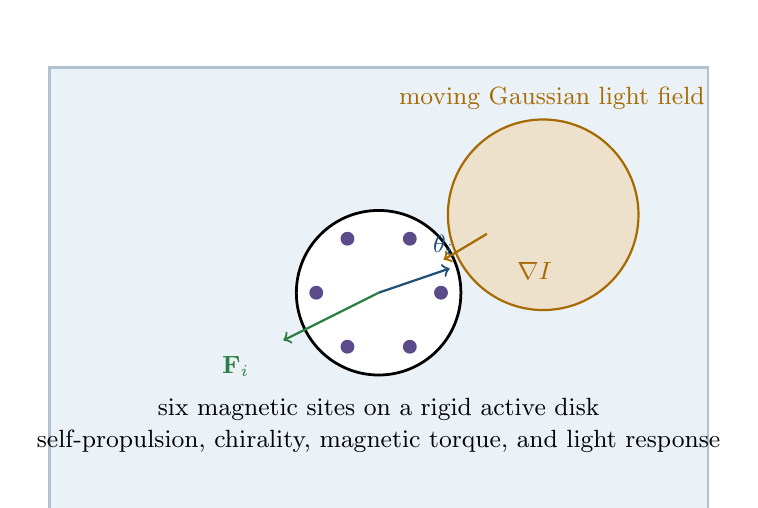
\begin{tikzpicture}[scale=1.1]
  \fill[SoftBlue] (-3.8,-2.6) rectangle (3.8,2.6);
  \draw[ReportBlue!35, line width=0.8pt] (-3.8,-2.6) rectangle (3.8,2.6);

  \fill[AccentAmber!20] (1.9,0.9) circle (1.1);
  \draw[AccentAmber, thick] (1.9,0.9) circle (1.1);
  \node[AccentAmber] at (2.0,2.25) {\small moving Gaussian light field};

  \draw[fill=white, line width=1pt] (0,0) circle (0.95);
  \draw[ReportBlue, thick, ->] (0,0) -- (0.82,0.28);
  \node[ReportBlue] at (0.75,0.55) {\small $\theta_i$};

  \foreach \ang in {0,60,120,180,240,300} {
    \fill[AccentPurple] ({0.72*cos(\ang)},{0.72*sin(\ang)}) circle (0.08);
  }

  \draw[AccentGreen, thick, ->] (0,0) -- (-1.1,-0.55);
  \node[AccentGreen] at (-1.65,-0.85) {\small $\mathbf{F}_i$};

  \draw[AccentAmber, thick, ->] (1.25,0.68) -- (0.75,0.38);
  \node[AccentAmber] at (1.8,0.25) {\small $\nabla I$};

  \node at (0,-1.35) {\small six magnetic sites on a rigid active disk};
  \node at (0,-1.72) {\small self-propulsion, chirality, magnetic torque, and light response};
\end{tikzpicture}
\caption{Schematic of the simulated Magbot model. The drawing was prepared for this report; the six-site active magnetic body and light-field control idea are conceptually inspired by the Robo-Matter Magbot system reported in Ref.~\cite{wang2024robomatter}.}
\label{fig:schematic}
\end{figure}

\runin{State variables}
For the $i$th Magbot, the main state variables are:

\begin{equation}
\mathbf{x}_i(t) = (x_i(t),y_i(t)), \qquad
\theta_i(t), \qquad
\phi_{ik}(t), \quad k=1,\ldots,N_{\mathrm{mag}}.
\end{equation}

Here $\mathbf{x}_i$ is the body-center position, $\theta_i$ is the body orientation, and $\phi_{ik}$ is the internal phase of the $k$th magnetic site. The fixed angular location of the $k$th site on the body is denoted by $\alpha_k$. The absolute magnet angle is therefore

\begin{equation}
\psi_{ik} = \theta_i + \alpha_k + \phi_{ik}.
\end{equation}

The six fixed anchor points are placed at radius $R_{\mathrm{ring}}$ from the center:

\begin{equation}
\mathbf{a}_k =
R_{\mathrm{ring}}
\begin{bmatrix}
\cos \alpha_k \\ \sin \alpha_k
\end{bmatrix},
\qquad
\alpha_k = \frac{2\pi(k-1)}{N_{\mathrm{mag}}}.
\end{equation}

\runin{Light field}
The simulation uses a Gaussian light field to represent a programmable activation pattern. For a light center $\mathbf{x}_L(t)$, the intensity at position $\mathbf{x}$ is

\begin{equation}
I(\mathbf{x},t) = I_0 + A_L
\exp\left[-\frac{\left|\mathbf{x}-\mathbf{x}_L(t)\right|^2}{2\sigma_L^2}\right].
\end{equation}

For the moving-spot case,

\begin{equation}
\mathbf{x}_L(t) = R_L
\begin{bmatrix}
\cos(2\pi t/T_L) \\
\sin(2\pi t/T_L)
\end{bmatrix}.
\end{equation}

The intensity is clipped to the interval $[0,1]$ in the implementation. The light affects both translational and rotational motion. It increases the active speed and changes the chiral angular velocity:

\begin{equation}
v_i = v_{\mathrm{base}} + \gamma I_i,
\end{equation}

\begin{equation}
\omega_i = \chi_i\left(\omega_{\mathrm{base}} + \beta I_i\right),
\end{equation}

where $\chi_i=-1$ denotes clockwise rotation and $\chi_i=+1$ denotes counterclockwise rotation.

\runin{Light-gradient drift}
The model includes a simplified drift toward brighter regions:

\begin{equation}
\mathbf{F}_{L,i} = k_L \nabla I(\mathbf{x}_i,t).
\end{equation}

For the Gaussian component,

\begin{equation}
\nabla I =
I_{\mathrm{spot}}
\frac{\mathbf{x}_L-\mathbf{x}}{\sigma_L^2}.
\end{equation}

This rule is not intended as a full electromechanical model of the real photoresistor-motor coupling. It is a compact way to represent light-guided activation and migration.

\runin{Magnetic interaction}
Each Magbot has six magnetic sites. For a pair of magnetic sites separated by vector $\mathbf{r}$ and distance $r$, the simulation uses the simplified interaction energy

\begin{equation}
U_{ab} =
-k_m \exp\left(-\frac{r^2}{r_0^2}\right)
\cos(\Delta\psi),
\end{equation}

where $k_m$ is magnetic strength, $r_0$ is the decay scale, and $\Delta\psi$ is the relative magnet-angle difference. The interaction is evaluated only when $r<r_{\mathrm{cut}}$.

The force contribution is obtained from the gradient of this potential. In the implemented form,

\begin{equation}
\mathbf{F}_{ab} =
\frac{2k_m}{r_0^2}
\exp\left(-\frac{r^2}{r_0^2}\right)
\cos(\Delta\psi)\,\mathbf{r}.
\end{equation}

The internal magnet phase torque is

\begin{equation}
\tau_{\phi} =
k_m
\exp\left(-\frac{r^2}{r_0^2}\right)
\sin(\Delta\psi).
\end{equation}

When a magnetic force acts away from the body center, it also creates body torque:

\begin{equation}
\tau_{\mathrm{body}} = \mathbf{r}_{\mathrm{lever}}\times\mathbf{F}.
\end{equation}

\runin{Steric repulsion and collision handling}
To prevent unphysical overlap, a hard-core repulsive force is applied when two disks overlap. If $d_{ij}$ is the center-to-center distance,

\begin{equation}
\mathbf{F}_{\mathrm{rep}} =
-k_{\mathrm{rep}}(2R_{\mathrm{bot}}-d_{ij})\hat{\mathbf{r}}_{ij},
\qquad d_{ij}<2R_{\mathrm{bot}}.
\end{equation}

After force-based integration, the code also performs direct overlap resolution through a few sweeps. This improves numerical stability in dense configurations.

\runin{Equations of motion}
The overdamped translational update is

\begin{equation}
\mathbf{x}_i(t+\Delta t) =
\mathbf{x}_i(t)
+
\left[
\mu_t\mathbf{F}_i
+\mathbf{F}_{L,i}
+v_i\mathbf{n}_i
\right]\Delta t
+\sqrt{2D_t\Delta t}\,\bm{\eta}_i,
\end{equation}

where $\mathbf{n}_i=(\cos\theta_i,\sin\theta_i)$ and $\bm{\eta}_i$ is a Gaussian random vector.

The body angle update is

\begin{equation}
\theta_i(t+\Delta t) =
\theta_i(t) +
\left[
\omega_i+\mu_r\tau_i
\right]\Delta t
+\sqrt{2D_r\Delta t}\,\xi_i.
\end{equation}

The internal magnet phase update is

\begin{equation}
\phi_{ik}(t+\Delta t) =
\phi_{ik}(t)+\mu_\phi \tau_{\phi,ik}\Delta t
+\sqrt{2D_\phi\Delta t}\,\zeta_{ik}.
\end{equation}

\section{Numerical Implementation and Analysis}
The main simulations use reflecting square boundaries. If a particle crosses a vertical wall, its orientation is reflected as

\begin{equation}
\theta \rightarrow \pi-\theta.
\end{equation}

If it crosses a horizontal wall,

\begin{equation}
\theta \rightarrow -\theta.
\end{equation}

The position is clipped inside the simulation box. This mimics elastic reflection at rigid boundaries.

\runin{Cell-list neighbor search}
Direct pairwise interaction checking scales as $O(N^2)$ and becomes inefficient for large $N$. The simulation therefore divides the domain into cells whose side length is comparable to the interaction cutoff. Each particle checks only particles in its own cell and neighboring cells. This keeps the interaction search efficient while preserving local pair detection.

\begin{keybox}{Computational design choice}
The cell-list method is important because the model contains both body-level and site-level interactions. Without local neighbor filtering, checking all possible site pairs for all Magbot pairs would become unnecessarily expensive.
\end{keybox}

\runin{Analysis metrics}
The results are analyzed using two complementary metrics.

\runin{Local topological order}
The local topological order parameter measures the degree of local structural organization. A high value indicates a stable neighborhood arrangement or locally ordered structure. In the plots generated for this project, a threshold line near $0.30$ separates low-order gas-like or fluid-like states from more ordered regimes.

\runin{Nearest-neighbor change rate}
The nearest-neighbor change rate $n_c$ measures how frequently the local neighborhood of particles changes. A low value indicates arrested or solid-like behavior, while a high value indicates frequent bond breaking and rearrangement. In the plots, a threshold line near $n_c=5$ is used as a practical separator between relatively stable and actively reorganizing structures.

\section{Simulation Cases}
Representative parameter choices used in the project are summarized in Table~\ref{tab:phaseparams}. These values are extracted from the simulation scripts in the \texttt{states} folder.

\begin{longtable}{>{\raggedright\arraybackslash}p{3.0cm}cccccc}
\caption{Representative parameter sets for four simulated Robo-Matter regimes.}
\label{tab:phaseparams}\\
\toprule
Regime & $N$ & box & $v_{\mathrm{base}}$ & $\omega_{\mathrm{base}}$ & $k_m$ & $r_0$ \\
\midrule
\endfirsthead
\toprule
Regime & $N$ & box & $v_{\mathrm{base}}$ & $\omega_{\mathrm{base}}$ & $k_m$ & $r_0$ \\
\midrule
\endhead
Active glass-like & 150 & 20.0 & 0.45 & 0.50 & 5.80 & 4.00 \\
Active crystal & 150 & 17.0 & 10.45 & 6.90 & 10.00 & 5.00 \\
Liquid-like & 100 & 20.0 & 6.50 & 5.80 & 2.50 & 0.95 \\
Gas-like & 100 & 28.0 & 10.00 & 10.00 & 0.80 & 0.80 \\
\bottomrule
\end{longtable}

% ------------------------------------------------------------
% Chapter 6
% ------------------------------------------------------------
\chapter{Theory}

\section{Active Brownian and Chiral Motion}
A minimal active Brownian particle has the dynamics

\begin{equation}
\dot{\mathbf{x}} = v_0 \mathbf{n}(t) + \sqrt{2D_t}\,\bm{\eta}(t),
\end{equation}

\begin{equation}
\dot{\theta} = \sqrt{2D_r}\,\xi(t).
\end{equation}

At short times, the particle keeps its direction and motion is approximately ballistic. At long times, rotational diffusion destroys directional memory and the motion becomes diffusive. This crossover is central to active matter.

\runin{Chiral extension}
For a chiral particle, an intrinsic angular velocity is added:

\begin{equation}
\dot{\theta} = \omega + \sqrt{2D_r}\,\xi(t).
\end{equation}

If noise and interaction are absent, the particle follows a circular trajectory with approximate radius

\begin{equation}
R_{\mathrm{circle}} = \frac{v_0}{|\omega|}.
\end{equation}

In the Robo-Matter simulation, chirality is important because Magbots in the experimental system rotate due to vibration motors and tilted brushes. The sign of $\omega$ controls clockwise or counterclockwise motion.

\runin{Mean squared displacement}
Although the primary project plots focus on structural order and neighbor-change rate, the theoretical mean squared displacement (MSD) remains a useful reference quantity. For a non-chiral ABP in two dimensions,

\begin{equation}
\langle \Delta r^2(t)\rangle =
4D_t t
+\frac{2v_0^2}{D_r^2}
\left(
D_r t + e^{-D_r t}-1
\right).
\end{equation}

For $t\ll D_r^{-1}$, the leading active contribution is approximately $v_0^2t^2$, indicating ballistic motion. For $t\gg D_r^{-1}$, the MSD becomes diffusive with an effective diffusion coefficient

\begin{equation}
D_{\mathrm{eff}} = D_t + \frac{v_0^2}{2D_r}.
\end{equation}

In interacting Robo-Matter, this simple expression is modified by magnetic binding, confinement, collision, and collective rearrangement. However, the ballistic-to-diffusive idea remains useful for interpreting activity-driven spreading.

\section{Phase Interpretation}
The phase behavior can be interpreted through a dimensionless qualitative ratio:

\begin{equation}
\Lambda =
\frac{k_m}{v_{\mathrm{base}}+\omega_{\mathrm{base}}+\epsilon},
\end{equation}

where $\epsilon$ prevents division by zero and reminds us that this is not a rigorous thermodynamic parameter. Large $\Lambda$ indicates strong binding compared with agitation. Small $\Lambda$ indicates weak binding compared with activity. In the project, this ratio is used conceptually rather than as a fitted universal order parameter.

\begin{table}[H]
\centering
\caption{Qualitative transition logic used to interpret simulated phases.}
\label{tab:transitionlogic}
\begin{tabularx}{\textwidth}{>{\bfseries}p{3.2cm}X X}
\toprule
Condition & Expected behavior & Representative phase \\
\midrule
Strong binding, low activity & Particles bind but cannot easily escape disordered local traps. & Active glass-like \\
Strong binding, moderate activity & Motion anneals defects while attraction maintains local order. & Active crystal \\
Comparable binding and activity & Bonds form and break continually; the network flows. & Liquid-like \\
Weak binding, high activity & Particles or small clusters roam independently. & Gas-like \\
\bottomrule
\end{tabularx}
\end{table}

\runin{Role of magnet symmetry}
Six magnetic sites produce a natural route to local hexagonal or honeycomb-like packing. The fixed body anchors introduce anisotropy: attraction depends not only on distance but also on relative magnet orientation. This makes the model richer than a simple isotropic Lennard-Jones-like attraction. Body torque and internal magnet torque allow local magnetic alignment to influence both individual particle orientation and collective structure.

\runin{Relation to experimental Robo-Matter}
The experimental paper reports that homogeneous light intensity can play a temperature-like role: stronger light increases Magbot activation and changes collective organization \cite{wang2024robomatter}. In this simulation, the light field increases active speed and rotation rate. Therefore, activity can melt stable clusters, promote reorganization, or disperse the system depending on magnetic binding strength.

% ------------------------------------------------------------
% Chapter 7
% ------------------------------------------------------------
\chapter{Results and Discussion}

\section{Phase-State Results}
The simulation produces four representative phase-like regimes. They are not thermodynamic phases in the strict equilibrium sense; they are nonequilibrium collective states distinguished by local order, bond rearrangement, density, and activity.

\begin{table}[H]
\centering
\caption{Interpretation of the simulated phase-like regimes. The phase names follow the Robo-Matter terminology introduced in Ref.~\cite{wang2024robomatter}, while the signatures reported here are obtained from this project's simulations.}
\label{tab:phaseinterpretation}
\begin{tabularx}{\textwidth}{>{\bfseries}p{3.0cm}X X}
\toprule
Regime & Structural signature & Dynamical signature \\
\midrule
Active glass-like & Locally connected or jammed structure with limited ability to rearrange globally. & Neighbor-change rate decays; motion becomes arrested. \\
Active crystal & High local order and stable neighborhood structure. & Defects are annealed; neighbor changes fall below threshold. \\
Liquid-like & Partial local order with continuous restructuring. & Neighbor changes remain frequent; bonds form and break. \\
Gas-like & Low topological order and mostly separated particles or small clusters. & Particles remain mobile and disordered. \\
\bottomrule
\end{tabularx}
\end{table}

\runin{Active crystal phase}
The active crystal simulation uses strong magnetic binding and sufficiently high motion to allow reorganization. Figure~\ref{fig:activecrystal} shows that the local topological order rises rapidly from a low value to above $0.8$ and remains high for most of the simulated time. The nearest-neighbor change rate initially spikes, corresponding to active rearrangement and defect correction, but then decreases below the threshold line.

\begin{figure}[H]
\centering
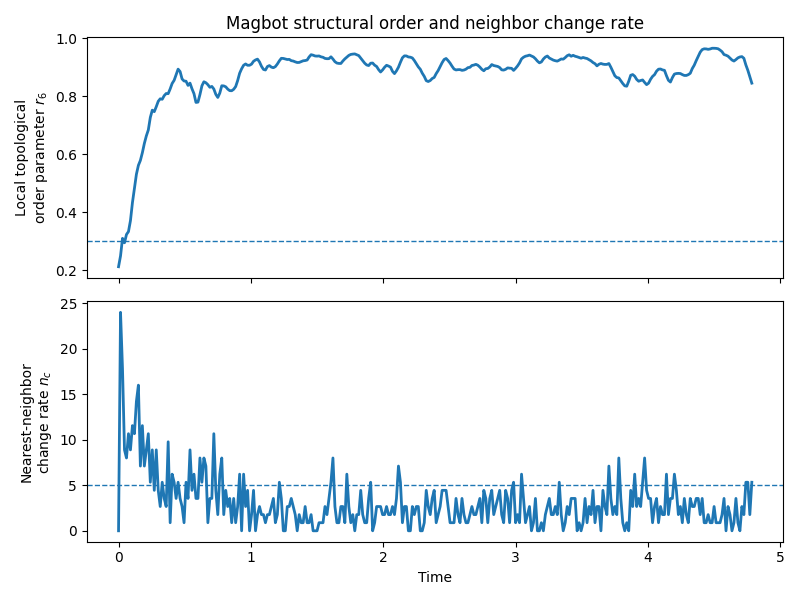
\includegraphics[width=0.92\textwidth]{active_crystal_phase.png}
\caption{Project-generated active-crystal simulation output. The local topological order rapidly becomes high, while the nearest-neighbor change rate decreases after initial rearrangement. The phase label is used in the qualitative sense of Ref.~\cite{wang2024robomatter}.}
\label{fig:activecrystal}
\end{figure}

\begin{resultbox}{Result highlight: active crystal}
The active crystal is produced when magnetic binding is strong but the system still has enough motion to anneal defects. In physical terms, activity is not merely destructive; at moderate levels it helps the system escape local disorder and settle into a more ordered state.
\end{resultbox}

\runin{Active glass-like phase}
The active glass-like case corresponds to strong attraction and low activity. Figure~\ref{fig:activeglass} shows a gradual increase in order and a decay of neighbor changes. The key distinction from an ideal active crystal is that rearrangement becomes suppressed before the system can fully explore configuration space. This is characteristic of a kinetically arrested state.

\begin{figure}[H]
\centering
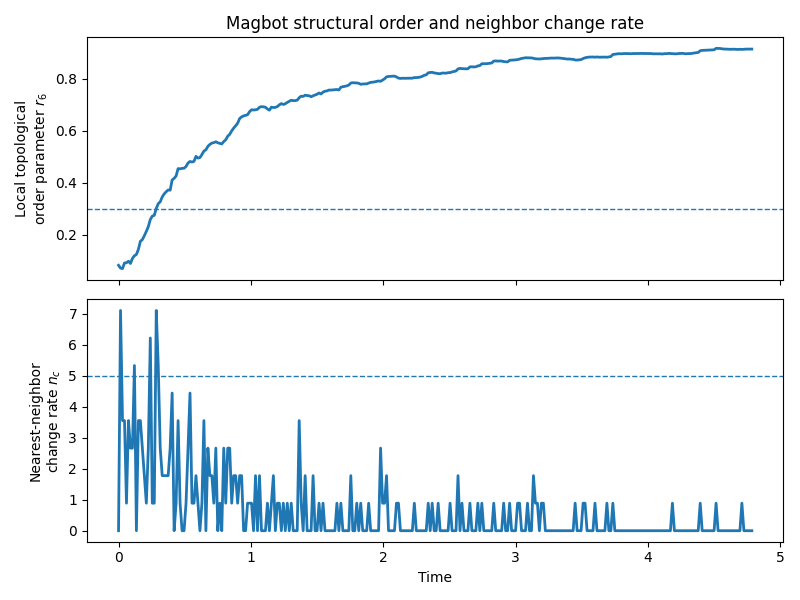
\includegraphics[width=0.92\textwidth]{active_glass_like.png}
\caption{Project-generated active glass-like simulation output. The system develops local organization, but the nearest-neighbor change rate decays strongly, indicating arrested dynamics and reduced ability to reorganize. The phase label follows the qualitative terminology of Ref.~\cite{wang2024robomatter}.}
\label{fig:activeglass}
\end{figure}

In the Robo-Matter interpretation, the glass-like state is not simply ``low order.'' It may contain local order but lacks sufficient rearrangement to remove defects or produce a clean crystalline structure. This agrees with the general physical idea that glassiness is associated with kinetic arrest.

\runin{Liquid-like phase}
The liquid-like simulation uses activity comparable to magnetic binding. Figure~\ref{fig:liquidlike} shows that local order grows gradually and eventually crosses the practical threshold, but the neighbor-change rate remains large and fluctuating. This is the defining signature of liquid-like behavior: local coordination exists, but bonds do not remain fixed.

\begin{figure}[H]
\centering
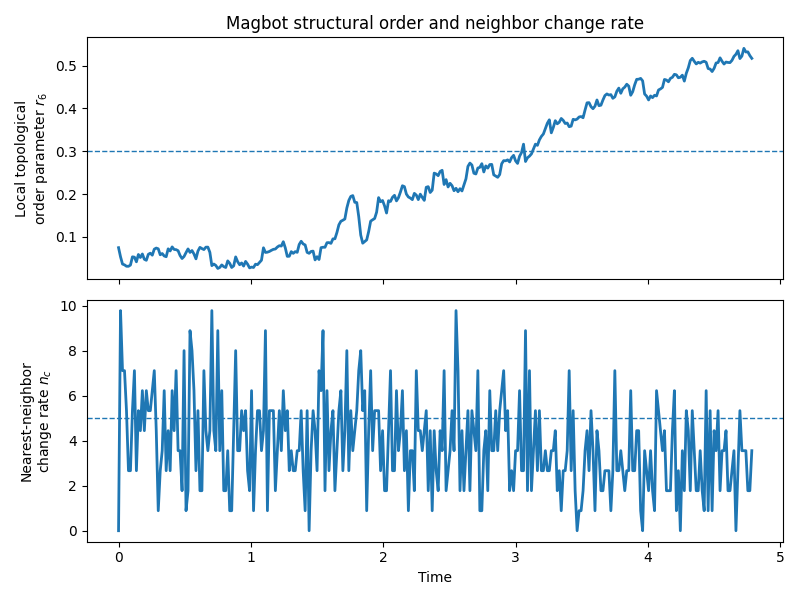
\includegraphics[width=0.92\textwidth]{liquid_like.png}
\caption{Project-generated liquid-like simulation output. Local order develops only gradually, while the nearest-neighbor change rate remains substantial. The phase label is used by analogy with the Robo-Matter regimes reported in Ref.~\cite{wang2024robomatter}.}
\label{fig:liquidlike}
\end{figure}

The liquid-like state is important because it demonstrates that collective organization need not be static. The particles can form temporary clusters and networks while continuously exchanging neighbors. This is similar to ordinary liquids, but here the motion is sustained by active drive rather than thermal equilibrium alone.

\runin{Gas-like phase}
In the gas-like regime, activity is high and magnetic attraction is weak. Figure~\ref{fig:gaslike} shows that the local topological order remains near zero and well below the threshold. Neighbor-change rate fluctuates because particles continue to encounter and separate from one another, but sustained binding is absent.

\begin{figure}[H]
\centering
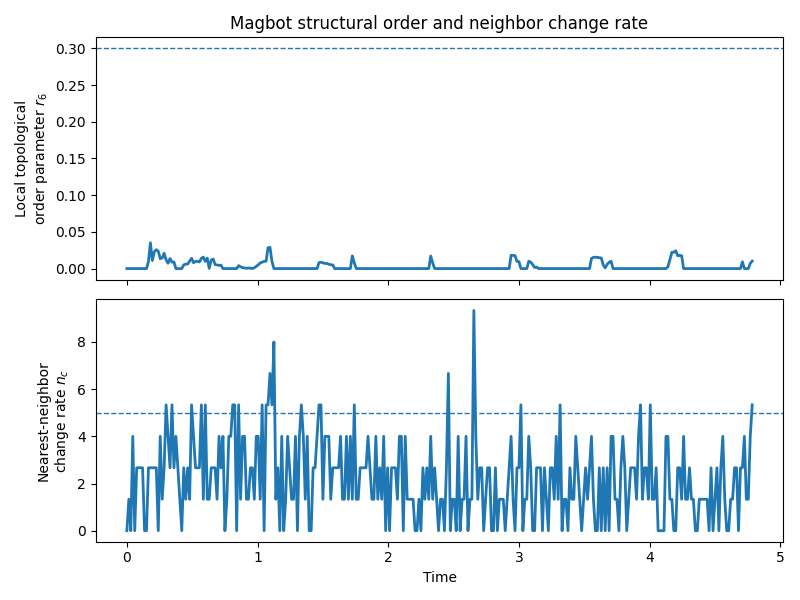
\includegraphics[width=0.92\textwidth]{gas_like_phase.png}
\caption{Project-generated gas-like simulation output. The order parameter remains very low, indicating absence of stable collective organization. Motion and weak binding lead to dispersed, disordered behavior. The phase label follows the qualitative framework of Ref.~\cite{wang2024robomatter}.}
\label{fig:gaslike}
\end{figure}

\section{Comparative Interpretation}
Figures~\ref{fig:activecrystal}--\ref{fig:gaslike} use the same visual format, axes, and diagnostic quantities, so they can be compared directly without shrinking the plots into a small multi-panel layout. The main simulation result is that changing the balance between activity, binding, and density changes the emergent Robo-Matter state.

\runin{Interpretation using order and dynamics}
The two selected metrics should be interpreted together. A high order parameter alone does not prove that the system is a good crystal, because a jammed state may also have local order. Similarly, a high neighbor-change rate alone does not prove disorder, because a liquid may have local structure while still rearranging. The useful classification is obtained by combining them:

\begin{table}[H]
\centering
\caption{Metric-based classification of collective states.}
\label{tab:metrics}
\begin{tabularx}{\textwidth}{>{\bfseries}p{3.2cm}X X}
\toprule
Metric combination & Physical meaning & Likely regime \\
\midrule
High order, low $n_c$ & Stable local structure with little rearrangement. & Active crystal or arrested glass \\
High/medium order, high $n_c$ & Structured but flowing network. & Liquid-like \\
Low order, high/medium $n_c$ & Disordered mobile particles or small clusters. & Gas-like \\
Low order, low $n_c$ & Frozen disordered state or insufficient motion. & Deep glass-like limit \\
\bottomrule
\end{tabularx}
\end{table}

\runin{Physical mechanism of transitions}
The transition sequence can be understood as:

\begin{equation}
\begin{aligned}
\text{glass-like}
&\xrightarrow{\text{increase activity}}
\text{active crystal}
\xrightarrow{\text{increase activity further}}
\text{liquid-like} \\
&\xrightarrow{\text{weak binding or high activity}}
\text{gas-like}.
\end{aligned}
\end{equation}

The first transition is subtle. A small increase in activity can improve order by allowing particles to escape trapped local configurations. However, too much activity breaks bonds faster than they can stabilize, producing liquid-like or gas-like behavior.

\runin{Comparison with experimental Robo-Matter}
The computational results are qualitatively consistent with the experimental Robo-Matter phase concept. In the experimental system, homogeneous light intensity affects Magbot rotation speed and plays a temperature-like role, while magnetic binding stabilizes assemblies \cite{wang2024robomatter}. The present simulation reproduces the same conceptual competition. It also includes a moving light field, allowing light-guided drift and activity modulation.

Important differences remain. The simulation does not model motor electronics, brush friction, real magnetic rod geometry, camera feedback, LED pixel control, or exact contact mechanics. Therefore, numerical values should not be interpreted as direct experimental predictions. The value of the model lies in mechanism-level understanding.

\section{Model Assessment}
The model is useful because it is physically interpretable: every term in the update rule corresponds to activity, force, torque, noise, or environmental control. It includes both translational and rotational dynamics, treats the internal magnet phases as active variables rather than fixed labels, reproduces four distinct collective regimes under parameter changes, and remains extendable because local neighbor search keeps the computation manageable.

The model is also deliberately simplified. The magnetic potential is not a full dipole-field calculation, friction and vibration-motor dynamics are represented phenomenologically, and the light-field drift is a compact control approximation rather than a detailed photo-electromechanical model. The order metrics are useful for this first study, but stronger quantitative phase classification would require longer simulations, multiple random seeds, additional structural metrics, and direct comparison with experimental datasets.

\section{Discussion}
The main scientific outcome of the project is the demonstration that Robo-Matter-like behavior can be generated from simple local rules. The simulations support the idea that active robotic materials should be understood as nonequilibrium many-body systems. Activity is not only a source of disorder; it can also enable reconfiguration, defect repair, and transition between states. Magnetic binding is not only a source of stability; if too strong relative to motion, it can arrest the system in a glass-like configuration. The useful operating regime for adaptive material behavior lies between these extremes.

% ------------------------------------------------------------
% Chapter 8
% ------------------------------------------------------------
\chapter{Conclusion}

\section{Summary, Limitations, and Future Directions}
This project developed a two-dimensional simulation framework for Robo-Matter inspired by active magnetic Magbot systems. Each Magbot was represented as a rigid circular disk with six magnetic sites, chiral rotation, active translational motion, light-field modulation, magnetic force, internal magnet torque, body torque, noise, steric repulsion, and reflecting boundaries. The simulation was implemented in Python and used cell-list neighbor search for efficiency.

The report followed the structure of a formal thesis study: introduction, literature review, rationale, objectives, methods, theory, results, discussion, conclusion, references, and appendices. The core results were organized around four phase-like regimes: active glass-like, active crystal, liquid-like, and gas-like.

The main findings can be summarized as follows. Strong magnetic binding with moderate activity supports ordered active-crystal-like behavior, whereas strong binding with insufficient rearrangement produces arrested glass-like behavior. When activity and binding become comparable, the system behaves like a liquid-like network in which bonds form and break persistently. When activity is high and magnetic binding is weak, the system becomes gas-like and dispersed. Across these cases, local topological order and nearest-neighbor change rate form a useful diagnostic pair because they separate static order from active rearrangement.

The project contributes a transparent computational platform for studying Robo-Matter. It connects experimental ideas from Magbot-based smart materials with explicit equations of motion and interpretable simulation outputs. Its limitations are the simplified magnetic potential, phenomenological light response, absence of detailed hardware mechanics, and limited statistical sampling. Future work should therefore perform systematic parameter sweeps over magnetic strength, activity, density, and noise; compute additional order parameters such as bond-orientational order, cluster-size distribution, radial distribution function, and MSD; use multiple random seeds; add feedback-controlled light fields; study different magnet symmetries and mixed chirality; and compare simulated phase diagrams more directly with experimental Robo-Matter data.

Robo-Matter is a powerful example of how material behavior can emerge from active, interacting building blocks. This project shows that even a simplified simulation can reproduce meaningful collective regimes and explain them through the balance of activity, magnetic binding, and dynamic rearrangement. The work therefore provides both a computational model and a conceptual bridge between active matter physics and reconfigurable robotic materials.

% ------------------------------------------------------------
% References
% ------------------------------------------------------------
\begin{thebibliography}{99}
\addcontentsline{toc}{chapter}{References}

\bibitem{wang2024robomatter}
J. Wang, G. Wang, H. Chen, Y. Liu, P. Wang, D. Yuan, X. Ma, X. Xu, Z. Cheng, B. Ji, M. Yang, J. Shuai, F. Ye, J. Wang, Y. Jiao, and L. Liu, ``Robo-Matter towards reconfigurable multifunctional smart materials,'' \textit{Nature Communications}, vol. 15, article 8853, 2024. doi: 10.1038/s41467-024-53123-6.

\bibitem{marchetti2013hydrodynamics}
M. C. Marchetti, J. F. Joanny, S. Ramaswamy, T. B. Liverpool, J. Prost, M. Rao, and R. A. Simha, ``Hydrodynamics of soft active matter,'' \textit{Reviews of Modern Physics}, vol. 85, pp. 1143--1189, 2013.

\bibitem{bechinger2016active}
C. Bechinger, R. Di Leonardo, H. Lowen, C. Reichhardt, G. Volpe, and G. Volpe, ``Active particles in complex and crowded environments,'' \textit{Reviews of Modern Physics}, vol. 88, 045006, 2016.

\bibitem{liebchen2017chiral}
B. Liebchen and D. Levis, ``Collective behavior of chiral active matter: pattern formation and enhanced flocking,'' \textit{Physical Review Letters}, vol. 119, 058002, 2017.

\bibitem{zottl2016active}
A. Zottl and H. Stark, ``Emergent behavior in active colloids,'' \textit{Journal of Physics: Condensed Matter}, vol. 28, 253001, 2016.

\bibitem{romanczuk2012active}
P. Romanczuk, M. Bar, W. Ebeling, B. Lindner, and L. Schimansky-Geier, ``Active Brownian particles: From individual to collective stochastic dynamics,'' \textit{European Physical Journal Special Topics}, vol. 202, pp. 1--162, 2012.

\bibitem{yang2024robomatter_supp}
Project source material, ``Robo-Matter simulation notes and Magbot modelling document,'' local file \texttt{robo\_matter.pdf}, BTP project folder, 2026.

\bibitem{projectcode}
Project simulation scripts, local files in \texttt{states/} and \texttt{updated/}, BTP project folder, 2026.

\end{thebibliography}

% ------------------------------------------------------------
% Appendices
% ------------------------------------------------------------
\appendix

\chapter{Simulation Parameters}

\section{Default Magbot Geometry}
\begin{table}[H]
\centering
\caption{Core geometric parameters used in the simulation.}
\begin{tabularx}{0.88\textwidth}{>{\bfseries}p{4.0cm}p{3.0cm}X}
\toprule
Parameter & Value & Meaning \\
\midrule
$N_{\mathrm{bots}}$ & 100--150 & Number of simulated Magbots \\
$N_{\mathrm{mag}}$ & 6 & Magnetic sites per Magbot \\
$R_{\mathrm{bot}}$ & 1.0 & Radius of each circular body \\
$R_{\mathrm{ring}}$ & 0.78 & Radius of the magnetic-site ring \\
$r_{\mathrm{mag}}$ & 0.105 & Visual/display radius of magnetic sites \\
\bottomrule
\end{tabularx}
\end{table}

\section{Common Numerical Parameters}
\begin{table}[H]
\centering
\caption{Common time integration and noise parameters.}
\begin{tabularx}{0.88\textwidth}{>{\bfseries}p{4.0cm}p{3.0cm}X}
\toprule
Parameter & Typical value & Meaning \\
\midrule
$D_t$ & 0.012 & Translational noise strength \\
$D_r$ & 0.025 & Rotational noise strength \\
$D_\phi$ & 0.012 & Internal magnet phase noise \\
$\mu_t$ & 1.0 & Translational mobility \\
$\mu_r$ & 0.50--0.55 & Rotational mobility \\
$\mu_\phi$ & 1.0 & Magnet phase mobility \\
$\Delta t$ & 0.003--0.015 & Time step \\
steps & 900--1600 & Number of frames/updates \\
seed & 7 & Random seed used in representative runs \\
\bottomrule
\end{tabularx}
\end{table}

\chapter{Mathematical Derivations}

\section{Euler-Maruyama Discretization}
For a stochastic differential equation

\begin{equation}
dX = a(X,t)\,dt + b\,dW_t,
\end{equation}

the Euler-Maruyama update is

\begin{equation}
X_{n+1} = X_n + a(X_n,t_n)\Delta t + b\sqrt{\Delta t}\,\eta_n,
\end{equation}

where $\eta_n$ is a standard normal random variable. This is the basis for the translational, rotational, and internal magnet phase updates used in the simulation.

\section{Torque from Off-Center Force}
For a force $\mathbf{F}=(F_x,F_y)$ applied at lever arm $\mathbf{r}=(r_x,r_y)$ from the center of a two-dimensional rigid body, the out-of-plane torque is

\begin{equation}
\tau_z = r_xF_y-r_yF_x.
\end{equation}

This expression is implemented through the \texttt{cross2d} helper function in the project scripts.

\chapter{Algorithm and Code Structure}

\section{Main Algorithm}
The simulation begins by initializing Magbot positions, body orientations, chirality values, and internal magnet phases. At every time step, the code computes the local light intensity and light gradient, builds a cell list for neighbor detection, evaluates steric repulsion and magnetic forces for nearby Magbot pairs, and computes the associated body and internal magnet torques. The positions, body angles, and magnet phases are then updated by Euler-Maruyama integration, followed by reflecting-wall handling and overlap resolution. The final part of each update refreshes visualization elements such as bodies, magnets, heading lines, light spots, and interaction lines, while the stored state is used for order and neighbor-change analysis.

\section{Representative Update Pseudocode}
\begin{lstlisting}[style=pythonstyle,caption={Simplified pseudocode representing the update logic used in the simulation.}]
for frame in range(steps):
    t = frame * dt

    I, gradI = light_intensity_and_gradient(pos, t)
    F, T_body, T_phi = compute_forces_and_torques(pos, theta, phi)

    n = np.column_stack((np.cos(theta), np.sin(theta)))
    v = v_base + v_light_gain * I
    omega = chirality * (omega_base + omega_light_gain * I)

    F_light = light_drift_strength * gradI

    pos += (mu_t * F + F_light + v[:, None] * n) * dt
    pos += np.sqrt(2.0 * Dt * dt) * rng.normal(size=pos.shape)

    theta += (omega + mu_r * T_body) * dt
    theta += np.sqrt(2.0 * Dr * dt) * rng.normal(size=len(theta))

    phi += mu_phi * T_phi * dt
    phi += np.sqrt(2.0 * Dphi * dt) * rng.normal(size=phi.shape)

    apply_reflecting_boundaries(pos, theta)
    resolve_overlaps(pos)
\end{lstlisting}

\section{Source Files Used}
\begin{table}[H]
\centering
\caption{Main local files used as project material.}
\begin{tabularx}{\textwidth}{>{\raggedright\arraybackslash}p{6.7cm}X}
\toprule
File & Role in the report \\
\midrule
\texttt{robo\_matter.pdf} & Explanation of Magbot variables, forces, torque, light field, and parameter meaning. \\
\texttt{Research Papers/s41467-024-53123-6...pdf} & Primary research paper on experimental Robo-Matter. \\
\texttt{states/active\_crystal\_phase.py} & Parameter set and code basis for active crystal simulation. \\
\texttt{states/active\_glass\_like.py} & Parameter set and code basis for glass-like simulation. \\
\texttt{states/liquid\_like.py} & Parameter set and code basis for liquid-like simulation. \\
\texttt{states/gas\_like\_phase.py} & Parameter set and code basis for gas-like simulation. \\
\texttt{states/*.png} & Figures included in the results section. \\
\href{\btptwogithub/states/first_video.mp4}{\texttt{states/first\_video.mp4}} & Simulation video stored with the project material. \\
\href{\btptwogithub}{BTP-2 GitHub folder} & Online repository folder containing the BTP-2 report, code, figures, and supporting material. \\
\bottomrule
\end{tabularx}
\end{table}

\chapter{Phase Notes}

\section{Parameter Influence}
The parameter response is consistent with the activation-versus-binding interpretation used throughout the report. Increasing $k_m$ promotes magnetic binding and local order, while increasing $r_0$ makes magnetic sites influence each other over a longer distance. Increasing $v_{\mathrm{base}}$ raises translational agitation, and increasing $\omega_{\mathrm{base}}$ strengthens chiral rotation, which can help rearrangement at moderate values but destabilize bonds when too large. Increasing the box size lowers density and reduces frequent clustering, while stronger noise tends to destroy order and move the system toward gas-like behavior.

\section{Transition Summary}
\begin{resultbox}{Final phase summary}
The simulated Robo-Matter states are controlled by the balance between magnetic binding and active agitation. Strong binding with enough rearrangement produces active crystals; strong binding with too little rearrangement produces glass-like arrest; comparable binding and activity produces liquid-like flow; weak binding under high activity produces gas-like dispersion.
\end{resultbox}

\end{document}
